\documentclass{article}
\textwidth=6in
\hoffset=0in
\voffset=0in

\usepackage{afterpage}
\usepackage{pgf}
\usepackage{tikz}
\usepackage{pdflscape}
\usetikzlibrary{arrows,automata}
\usepackage[latin1]{inputenc}
\usepackage{ngerman}
\usepackage[a4paper, total={6in, 8in}]{geometry}
\usepackage{amsmath}
\usepackage{amssymb}
\usepackage{stmaryrd}
\usepackage{graphicx}
\usepackage{tikz}
\usetikzlibrary{automata, arrows, fit, calc}
\usepackage{pifont}
\usepackage{amssymb}
\usepackage{gensymb}
\usepackage[ampersand]{easylist}


\newcommand{\gap}{\ \\ \\}
\newcommand{\chart}[6]{
    \node[round, 
          minimum width=#5, 
          minimum height=#6] (#1) at (#3,#4) {chart};
    \node[rect] (#2) at (#3,#4) {title};
}
\newcommand{\sepline}[2]{
}

% needs to be updated
\author{Max Springenberg, 177792\\
        Daniel Sonnabend, 190748}
\title{\
    ES "Ubungsblatt 2\\
    Gruppe Fr. 8-10
    }
\setcounter{section}{1}
\date{}

\begin{document}

\maketitle
\newpage

\subsection{Nennen Sie mindestens zwei Anforderungen an Spezifikations- und 
            Modellierungssprachen f"ur eingebettete Systeme.}

Zu den in der Vorlesung vorgestelleten Anforderungen an Spezifiations- und 
    Modellierungssprachen f"ur eingebettete Systeme sind:\\
\begin{enumerate}
    \item Hierarchy
    \item Component-based design
    \item Timing
    \item Support design reactive systems
        \subitem event-handling/ state und error orientiertes Verhalten
\end{enumerate}
\begin{landscape}
\subsection{}
Konventionen zur Notation:\\
Z sei die Bier-, G die Geschmacks- und F die Flaschentaste. F"ur den 
    Alkoholgehalt wird `nxA` in den Transitionen benutzt, was das n-malige
    Dr"ucken der Alkoholtaste A repr"asentiert.\\
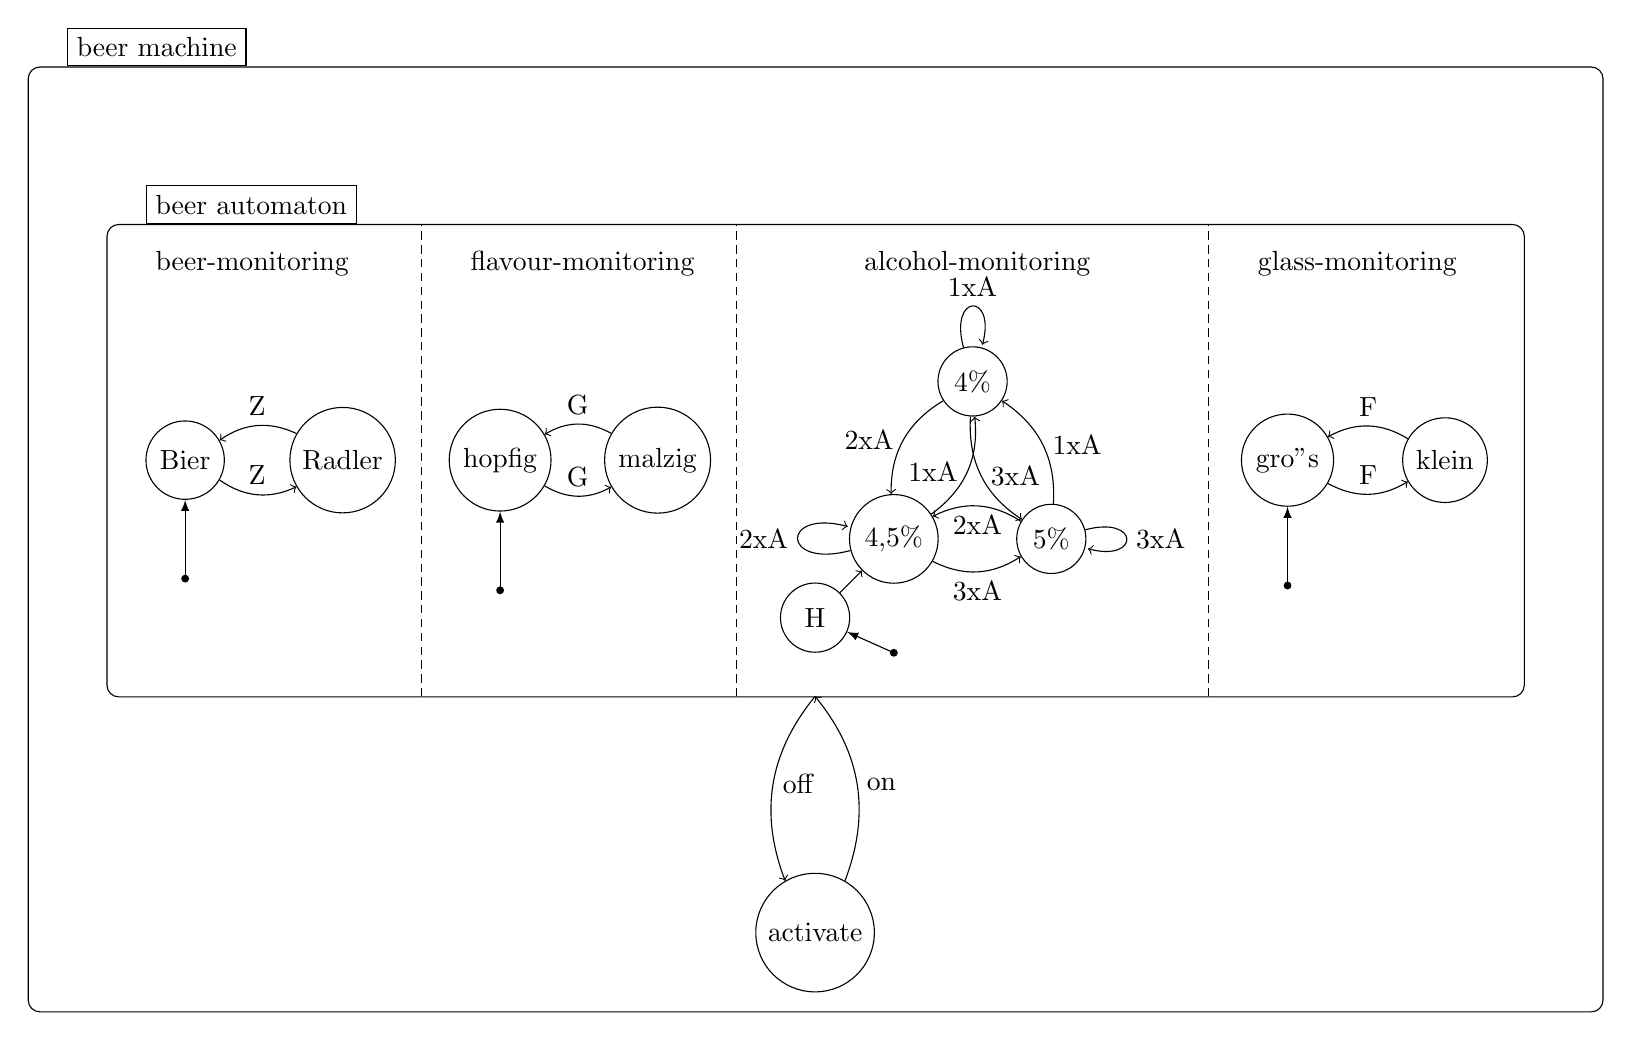
\begin{tikzpicture}[round/.style={rounded corners=1.5mm,minimum width=3cm,draw,
                                  anchor=north west},
                    rect/.style={draw, anchor=south west},
                    node distance =1cm]
    \node[anchor=west] (bierTitle) at (-0.5,2.5) {beer-monitoring};
    \node[state] (bier) at (0,0) {Bier};
    \node[state] (radler) at (2,0) {Radler};

    \node[anchor=west] (hopfigTitle) at (3.5,2.5) {flavour-monitoring};
    \node[state] (hopfig) at (4,0) {hopfig};
    \node[state] (malzig) at (6,0) {malzig};

    \node[anchor=west] (hopfigTitle) at (13.5,2.5) {glass-monitoring};
    \node[state] (gross) at (14,0) {gro"s};
    \node[state] (klein) at (16,0) {klein};

    \node[anchor=west] (hopfigTitle) at (8.5,2.5) {alcohol-monitoring};
    \node[state] (4) at (10,1) {4\%};
    \node[state] (45) at (9,-1) {4,5\%};
    \node[state] (H) at (8,-2) {H};
    \node[state] (5) at (11,-1) {5\%};

    \node[state] (active) at (8,-6) {activate};

    % chart beer automaton
    \node[round, 
          minimum width=18cm, 
          minimum height=6cm] (ba) at (-1,3) {};
    \node[rect] (baT) at (-0.5,3) {beer automaton};
    \draw[densely dashed] (3,-3) -- (3,3);
    \draw[densely dashed] (7,-3) -- (7,3);
    \draw[densely dashed] (13,-3) -- (13,3);
    % defaults
    % gross
    \draw[-latex] (gross.south) + (0,-1) coordinate (temp) to (gross);
        \fill (temp) circle (0.05);
    % hopfig
    \draw[-latex] (hopfig.south) + (0,-1) coordinate (temp) to (hopfig);
        \fill (temp) circle (0.05);
    % 4,5%/ H
    \draw[-latex] (H.south) + (1,0) coordinate (temp) to (H);
        \fill (temp) circle (0.05);
    % bier
    \draw[-latex] (bier.south) + (0,-1) coordinate (temp) to (bier);
        \fill (temp) circle (0.05);

    % chart machine
    \node[round, 
          minimum width=20cm, 
          minimum height=12cm] (bm) at (-2,5) {};
    \node[rect] (bmT) at (-1.5,5) {beer machine};

    % automata
    \path
        (bier)   edge [->, bend right, above] node {Z} (radler)
        (radler) edge [->, bend right, above] node {Z} (bier)

        (hopfig) edge [->, bend right, above] node {G} (malzig)
        (malzig) edge [->, bend right, above] node {G} (hopfig)

        (klein) edge [->, bend right, above] node {F} (gross)
        (gross) edge [->, bend right, above] node {F} (klein)

        (4) edge [->, loop above] node {1xA} (4)
        (4) edge [->, bend right, left] node {2xA} (45)
        (4) edge [->, bend right, right] node {3xA} (5)
        (45) edge [->, bend right, left] node {1xA} (4)
        (45) edge [->, loop left] node {2xA} (45)
        (45) edge [->, bend right, below] node {3xA} (5)
        (5) edge [->, bend right, right] node {1xA} (4)
        (5) edge [->, bend right, below] node {2xA} (45)
        (5) edge [->, loop right] node {3xA} (5)
        (H) edge [->] node {} (45)

        (active) edge [->, bend right, right] node {on} (8,-3) 
        (8, -3) edge [->, bend right, right] node {off} (active)
        ;
\end{tikzpicture}
\end{landscape}
\newpage

\subsection{}
(i)\\
\begin{tabular}{l|l|l|l}
    Zeit    &$e_1$   &$e_2$      & $a_1$ or $a_2$\\
    \hline
    0       &6       &0          & $a_1$\\
    1       &3       &2          & $a_1$\\
    2       &0       &4          & $a_2$\\
    3       &6       &0          & $a_1$\\
    4       &3       &2          & $a_1$\\
\end{tabular}\\
\gap
(ii)\\
\begin{tabular}{l|l|l|l}
    Time    &$e_1$   &$e_2$      & $a_1$, $a_2$ or ($a_1$ and $a_2$)\\
    \hline
    0       &9       &0          & $a_1$\\
    1       &6       &2          & $a_1$\\
    2       &3       &4          & $a_1$ and $a_2$\\
    3       &6       &2          & $a_1$\\
    4       &3       &4          & $a_1$ and $a_2$\\
\end{tabular}

\subsection{}
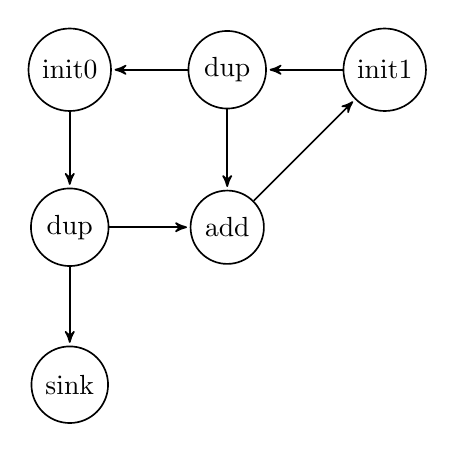
\begin{tikzpicture}[->,>=stealth',shorten >=1pt,auto,node distance=2.8cm,
                    semithick]
  %\tikzstyle{every state}=[fill=red,draw=none,text=white]

  \node[state] (init0)  at (0,0) {init0};
  \node[state] (init1)  at (4,0) {init1};
  \node[state] (dup0)   at (2,0) {dup};
  \node[state] (dup1)   at (0,-2) {dup};
  \node[state] (add)    at (2,-2) {add};
  \node[state] (sink)   at (0,-4) {sink};

  \path (init0) edge node {} (dup1)
        (init1) edge node {} (dup0)
        (dup0) edge node {} (init0)
               edge node {} (add)
        (dup1) edge node {} (add)
               edge node {} (sink)
        (add) edge node {} (init1);
\end{tikzpicture}
\end{document}
